\documentclass[10pt,a4paper]{report}
\usepackage[margin=1.25in]{geometry}
\usepackage{fancyhdr}
\usepackage[pdftex]{graphicx}
\usepackage{subfigure}
\usepackage{titlesec}
\usepackage{placeins}
\usepackage{color}
\usepackage{verbatim}
\usepackage{hyperref}
\usepackage{tikz}
\usepackage{pgf}
\usepackage{float}
\usepackage{hyperref}
\usepackage{multicol}
\usepackage{comment}

\usepackage{lipsum}
\usepackage{microtype}
\usepackage{vwcol}

\setlength{\columnseprule}{1pt}
\def\columnseprulecolor{\color{black!0}}

\usetikzlibrary{arrows,shapes,positioning,shadows,trees,automata}

\tikzset{
  basic/.style  = {draw, text width=2cm, drop shadow, font=\sffamily, rectangle},
  root/.style   = {basic, rounded corners=2pt, thin, align=center,
                   fill=green!30},
  level 2/.style = {basic, rounded corners=6pt, thin,align=center, fill=orange!30,
                   text width=10em},
  level 3/.style = {basic, thin, align=left, fill=pink!60, text width=11em, align=center},
	level 4/.style = {basic, thin, align=left, fill=pink!60, text width=14.5em, align=center},
	level 5/.style = {basic, thin, align=left, fill=pink!60, text width=6.5em, align=center}
}

\hypersetup{
    colorlinks=true,
    linkcolor=blue,
    citecolor=blue,
    filecolor=black,
    urlcolor=blue
}

\author{CC-Staff}
\title{User Documentation}
\date{8 May 2018}

\makeatletter
\let\thetitle\@title
\let\theauthor\@author
\let\thedate\@date
\makeatother

\pagestyle{fancy}
\fancyhf{}
\rhead{\theauthor}
\lhead{DCRAB User Guide}
\cfoot{\thepage}

\titleformat{\chapter}
  {\normalfont\LARGE\bfseries}{\thechapter}{1em}{}
\titlespacing*{\chapter}{0pt}{3.5ex plus 1ex minus .2ex}{2.3ex plus .2ex}


\begin{document}

%%%%%%%%%%%%%%%%%%%%%%%%%%%%%%%%%%%%%%%%%%%%%%%%%%%%%%%%%%%%%%%%%%%%%%%%%%%%%%%%%%%%%%%%%

\begin{titlepage}
	\centering
    \vspace*{3 cm}
    
\includegraphics[scale = 0.6]{../auxFiles/logos/DCRAB_logo.png}\\[1.0 cm]
		\vspace*{2 cm}
	\rule{\linewidth}{0.2 mm} \\[0.4 cm]
	{ \huge \bfseries \thetitle}\\
	\rule{\linewidth}{0.2 mm} \\[0.4 cm]
\vspace*{4.5 cm}
	\begin{minipage}{0.4\textwidth}
		\begin{flushleft} \large
			Document Revision 1.0\\
			8 May 2018\\
			\end{flushleft}
			\end{minipage}
			\begin{minipage}{0.4 \textwidth}
			\begin{flushright} \large
			DCRAB v2.0\\
		\end{flushright}
	\end{minipage}\\[2 cm]

%%%%%%%%%%%%%%%%%%%%%%%%%%%%%%%%%%%%%%%%%%%%%%%%%%%%%%%%%%%%%%%%%%%%%%%%%%%%%%%%%%%%%%%%%
\newpage
\thispagestyle{empty}
\begin{flushleft}
CC-Staff \\
Contact: http://dipc.ehu.es/cc/computing\_resources/staff.html \\
High Performance Computing \\
Donostia International Physics Center, Computing Center \\
Donostia - San Sebasti\'an \\
\vspace{1cm}
DCRAB Copyright (C) 2018 CC-Staff
\end{flushleft}

\newpage
\end{titlepage}

%%%%%%%%%%%%%%%%%%%%%%%%%%%%%%%%%%%%%%%%%%%%%%%%%%%%%%%%%%%%%%%%%%%%%%%%%%%%%%%%%%%%%%%%%

\begin{abstract}

DCRAB is a tool to monitorize resource utilization in HPC environments. It works side-by-side with the job scheduler to collect runtime information about the processes generated in the compute nodes.

Excluding a few cases, the data DCRAB collects is taken from the processes which the job has started, not from the entire node. The tool is able to collect the information listed below:

\begin{itemize}
	\item CPU used
	\item Memory usage
	\item Infiniband statistics (of the entire node)
	\item Processes IO statistics
	\item NFS usage (of the entire node)
	\item Disk IO statistics
\end{itemize}

\end{abstract}

%%%%%%%%%%%%%%%%%%%%%%%%%%%%%%%%%%%%%%%%%%%%%%%%%%%%%%%%%%%%%%%%%%%%%%%%%%%%%%%%%%%%%%%%%

\tableofcontents

%%%%%%%%%%%%%%%%%%%%%%%%%%%%%%%%%%%%%%%%%%%%%%%%%%%%%%%%%%%%%%%%%%%%%%%%%%%%%%%%%%%%%%%%%

\chapter{Installation}

DCRAB has no installation at all, you have to take the lastest version tarball available in Github (currently v2.0) and expand it in a convenient location in your system:

\begin{verbatim}
    tar xzvf ./DCRAB-2.0.tar.gz
\end{verbatim}

This will create a directory called \verb+DCRAB-2.0+ with some subdirectories:

\begin{itemize}
  \item \verb+/auxFiles+ which is used to store the auxiliary files useful for the internal operation mode of the tool as described in \ref{internalReport} section.
  \item \verb+/config+ folder which only contains a folder to store the current version of the tool.
  \item \verb+/docs+ which contains this documentation and the \verb+.tex+ used to generate.
  \item \verb+/examples+ is used to stored DCRAB's generated report examples of each version since it was created.
  \item \verb+/src+ folder contains the source files of the tool. Inside you will find \verb+dcrab+ script, which is the script that launches DCRAB and a folder called \verb+/script+ that contains the other scripts used by the tool to work.
\end{itemize}

Also you will find the \verb+readme.md+ file and the GNU GPL 3.0 license file \verb+COPYING+.

\chapter{Using DCRAB}

\section{Data Collection}
\label{dataCollection}
DCRAB has two operation modes: normal report operation, which may be the mode used by non-admin users, and internal report operation, which is focused to sysadmins. The second operation mode is going to be explained in \ref{internalReport} section, so firstly we will introduce here the normal report operation which will be the commonly used one.

The tool is straightforward to use, you have to add the following lines into your submission script:

\begin{verbatim}
    export DCRAB_PATH=/PATH_TO_DCRAB/src/
    export PATH=$PATH:$DCRAB_PATH
    dcrab start

    ##################################
    #    BLOCK OF CODE TO MONITOR    #
    ##################################

    dcrab finish
\end{verbatim}

Note that the variable \verb+DCRAB_PATH+ must be declared to run DCRAB and always must point to \verb+/src+ folder of the tool.

DCRAB will start a process in each compute node where the script runs, and will monitorize the processes started by it. The script will run as normal, and meanwhile DCRAB will generate a directory report called \verb+dcrab_report_<jobid>+ where \verb+jobid+ is the job number assigned by the scheduler. This reporting directory is generated in the same folder where the job was submitted.

\sloppy Inside this reporting directory, DCRAB will create the reporting file called \verb+dcrab_report.html+, which will be named as "the reporting file" is this document from now on. Generate this file is the main purpose of this monitorization and there you will find statistics and plots to analyze visually the information collected. This report is continuous change (every 10 seconds by default) because the information collected is stored at the time it is taken. So, you could open it with a browser, at the start of the job's execution, and refresh to see what is going on with the job.

One of the goals was to provide a single file to visualize all the data monitorized. So, the reporting file is completely modular and you can copy or move it to any location because every plot and image is embedded in the report.

To conclude, say that inside the \verb+dcrab_report_<jobid>+ reporting folder you will find some subdirectories, which normally are not relevant at all for the user because they are generated to guarantee the correct behaviour of the tool. One will be \verb+/data+, which contains for each computing node the files in charge of the management of the processes asociated with the job. Another folder called \verb+/auxFile+ stores the files used for the comunication between compute nodes, and \verb+/log+, which contains the output generated by DCRAB process in each node and DCRAB's main process output (all used for troubleshooting).

\section{Execution Customization}

In DCRAB version 2.0 is not included yet any configuration file to customize the execution, but it is included in the roadmap. However, there are some variables that could be changed inside the code until the configuration file is released:

\begin{itemize}
	\item \texttt{DCRAB\_COLLECT\_TIME}: this variable, inside \verb+src/scripts/dcrab_config.sh+ in \texttt{dcrab\_init\_variables()} function, configures the time between each data collection. By default it is set to 10 seconds.
	\item \texttt{DCRAB\_NFS\_MOUNT\_PATH}: this variable configures the path of the NFS filesystem to be monitorized. It is inside \verb+src/scripts/dcrab_node_monitoring_functions.sh+ in \texttt{dcrab\_node\_monitor\_init\_variables()} function. By defaut its value is \verb+/scratch+.
\end{itemize}

\section{Crashed Jobs}
\label{crash}
Update the reporting file continuosly imposed some troubles but it was one of our first goals. There is no much problem for the tool when the job crashes because the report has been generating until that moment, so it brings you such a great trace of what has been occurred and it may contain relevant information about the crash.

On the other hand, the tool by itself throws errors when some situations occur and has different exit codes for each one:

\begin{itemize}
	\item EXIT CODE 0, the tool exited normally and without errors.
	\item EXIT CODE 1, when \texttt{DCRAB\_PATH} is not defined.
	\item EXIT CODE 2, when there is an error in the tool invocation (e.g. 'dcrab stat' and no 'dcrab start').
	\item EXIT CODE 3, when the tool waited too much for the \texttt{control\_port.txt} file to be created.
	\item EXIT CODE 4, when some of the compute nodes try to write so many times in the reporting file with no success.
	\item EXIT CODE 5, when the reporting directory has been deleted or moved.
	\item EXIT CODE 6, when \texttt{DCRAB\_USER\_PROCESSES\_FILE} can not be read.
\end{itemize}

In this cases, a file called \verb+DCRAB_ERROR_<computeNodeHostname>_<jobid>+ will be generated, per each compute node involved in the calculation, in the same folder as the reporting folder: where the job was submitted. The \verb+computeNodeHostname+ refers to the hostname of the compute node that throws the error and \verb+jobid+ is the job number assigned by the scheduler to the job.


\chapter{Design and Implementation}

The main idea of DCRAB was to create a tool easy to use for the users. Notwithstanding that DCRAB is upgrading an HTML file continuosly, the runtime penalty is superfluous.

The continue upgrading of the report conditioned and formed DCRAB's structure. This upgrade is a critical section of the project because all the compute nodes need to write there at the same time, so there is a race condition we had to solve. In early versions we resolved the problem with a lock, to make the writing as an atomic operation, but there was a problem with the delay of parallel filesystems when the reporting file become bigger. The error was when a compute node wrote in the report file. In those writings some data was lost because there is a little delay until the file is upgraded or refreshed with the new information for other nodes. The unique way to solve the problem was to serialize those writings (using a mark in the first line of the report), to be sure one node wrote after the previous node had written.

In its current implementation the tool makes a ssh from the master node to all other nodes. This connection starts a process in background that monitorizes the processes started by the job and collects information about them (every 10 seconds by default). The tool take advantage of the scheduler to know which processes are related to that job.

\section{Statistics Collected}

DCRAB collects different statistics and information which may be usefull for the user. Here is the complete list of these statistics:

\begin{itemize}
	\item \textbf{CPU used}. The application reports the CPU usage for all the processes started by the job. This data is collected with \verb+ps+ command so it is a snapshot of the process at a concrete time. To have only a view of the main processes in the chart there is a threshold value defined to avoid trivial processes of the user. This information is very useful for applications that use OpenMP.
	\item \textbf{Memory usage}. This value is obtained with the processes' \verb+/proc/<pid>/status+ file where \verb+pid+ is the PID of the process. The tool collect information about Virtual Memory (displayed as VmSize), Resident Memory and Max Resident Memory (displayed as VmRSS). Also is displayed the memory requested by the user for that job in the scheduler and the total memory available in the node.

	If there are more than one node involved in the execution a bigger pie chart is generated to display the amount of memory used for the scheduler (with one node calculation this value is the same as the usage in that node so there is no reason to generate this plot). With this information the users could revise the amount of memory requested into a more real value one to not waste resources, which may also help schedulers' algorithms such as \verb+Backfill+ of Moab.
	\item \textbf{Infiniband statistics (of the entire node)}. There is counted the number of packets and MB of data transfered and received over Infiniband in the entire node (this values can not be collected per processes). This information can be used to improve or revise certain parts of the code, reducing the amount of data transferred over the network, comparing this code section with high network activity levels. This values are taken from the counters available in \verb+/sys/class/infiniband/mlx5_0/ports/1/counters+.
	\item \textbf{Processes IO statistics}. The I/O (Input/Output) made by the processes (regardless of the type of the filesystem). This information can be useful to see if a process is writing more than expected which could be a bottleneck in the program. This data is collected from \verb+/proc/<pid>/io+ file where \verb+pid+ is the PID of the process.
	\item \textbf{NFS usage (of the entire node)}. The I/O (Input/Output) made by the processes on the NFS filesystem determined by \verb+DCRAB_NFS_MOUNT_PATH+ variable. This value, as the Infiniband value, can not be measured by process and must be a collected from the entire node statistics. The information is collected from \verb+mountstats+ command.
	\item \textbf{Disk IO statistics (of the entire node)}. The I/O (Input/Output) made by the processes on the local disks. This data is obtained from \verb+/proc/diskstats+ file so this value is from to the entire node and not only of the current job.
\end{itemize}

\section{Code Structure}

This are the scripts that compose DCRAB. Here does not appear the internal report operation scripts, which are dcrab\_internal\_report\_generation.sh and dcrab\_internal\_report\_functions.sh, because will be explained in \ref{internalReportChapter} chapter.

\vspace*{1.5 cm}

\begin{figure}[H]
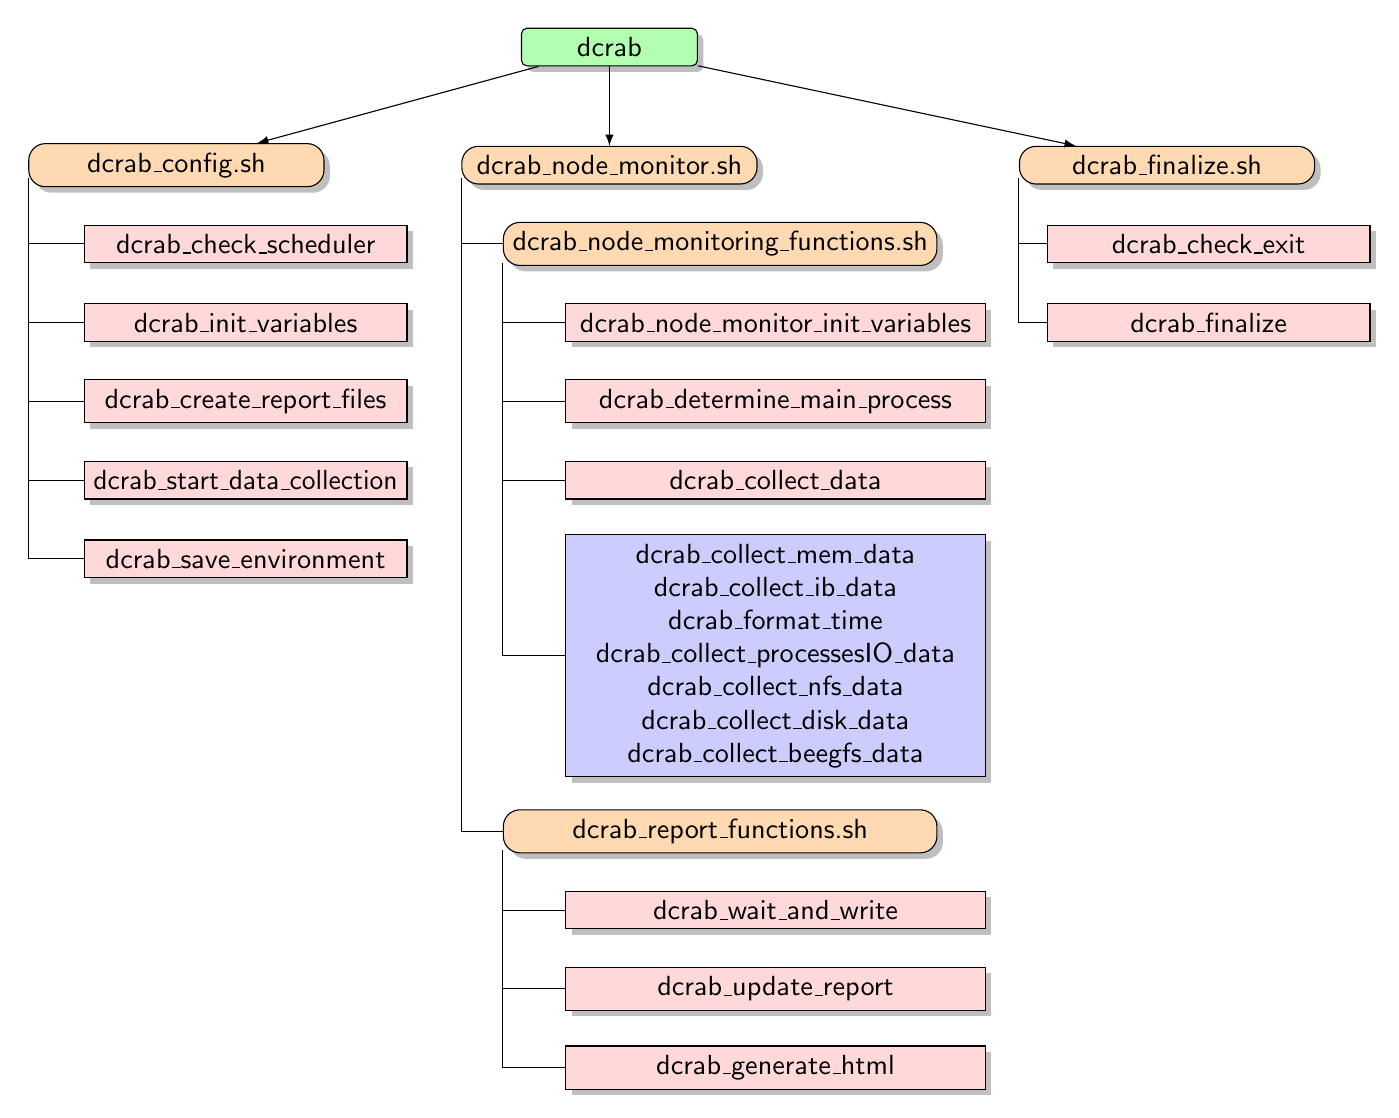
\begin{tikzpicture}[
  level 1/.style={sibling distance=55mm},
  edge from parent/.style={->,draw},
  >=latex]

% root of the the initial tree, level 1
\node[root] {dcrab}
% The first level, as children of the initial tree
  child {node[level 2] (c1) {dcrab\_config.sh}}
  child {node[level 2] (c2) {dcrab\_node\_monitor.sh}}
	child {node[level 2, xshift=45pt] (c3) {dcrab\_finalize.sh}};

% The second level, relatively positioned nodes
\node [level 3, below of = c1, xshift=25pt] (c11) {dcrab\_check\_scheduler};
\node [level 3, below of = c11] (c12) {dcrab\_init\_variables};
\node [level 3, below of = c12] (c13) {dcrab\_create\_report\_files};
\node [level 3, below of = c13] (c14) {dcrab\_start\_data\_collection};
\node [level 3, below of = c14] (c15) {dcrab\_save\_environment};

\node [level 3, below of = c2, xshift=40pt, rounded corners=6pt, fill=orange!30, text width=15em] (c21) {dcrab\_node\_monitoring\_functions.sh};
\node [level 4, below of = c21, xshift=20pt] (c211) {dcrab\_node\_monitor\_init\_variables};
\node [level 4, below of = c211] (c212) {dcrab\_determine\_main\_process};
\node [level 4, below of = c212] (c213) {dcrab\_collect\_data};
\node [level 4, below of = c213, yshift=-35pt, fill=blue!20] (c214) {dcrab\_collect\_mem\_data \\ dcrab\_collect\_ib\_data \\ dcrab\_format\_time \\ dcrab\_collect\_processesIO\_data \\ dcrab\_collect\_nfs\_data \\ dcrab\_collect\_disk\_data \\ dcrab\_collect\_beegfs\_data };

\node [level 3, below of = c214, xshift=-20pt, yshift=-35pt, rounded corners=6pt, fill=orange!30, text width=15em] (c22) {dcrab\_report\_functions.sh};
\node [level 4, below of = c22, xshift=20pt] (c221) {dcrab\_wait\_and\_write};
\node [level 4, below of = c221] (c222) {dcrab\_update\_report};
\node [level 4, below of = c222] (c223) {dcrab\_generate\_html};

\node [level 3, below of = c3, xshift=15pt] (c31) {dcrab\_check\_exit};
\node [level 3, below of = c31] (c32) {dcrab\_finalize};

\foreach \value in {1,...,5}
  \draw[-] (c1.185) |- (c1\value.west);
\foreach \value in {1,2}
	\draw[-] (c2.185) |- (c2\value.west);
\foreach \value in {1,2,3,4}
	\draw[-] (c21.185) |- (c21\value.west);
\foreach \value in {1,2,3}
	\draw[-] (c22.185) |- (c22\value.west);
\foreach \value in {1,2}
	\draw[-] (c3.185) |- (c3\value.west);
\end{tikzpicture}
\caption{DCRAB's code structure}
\label{codeTree}
\end{figure}

\begin{figure}[H]
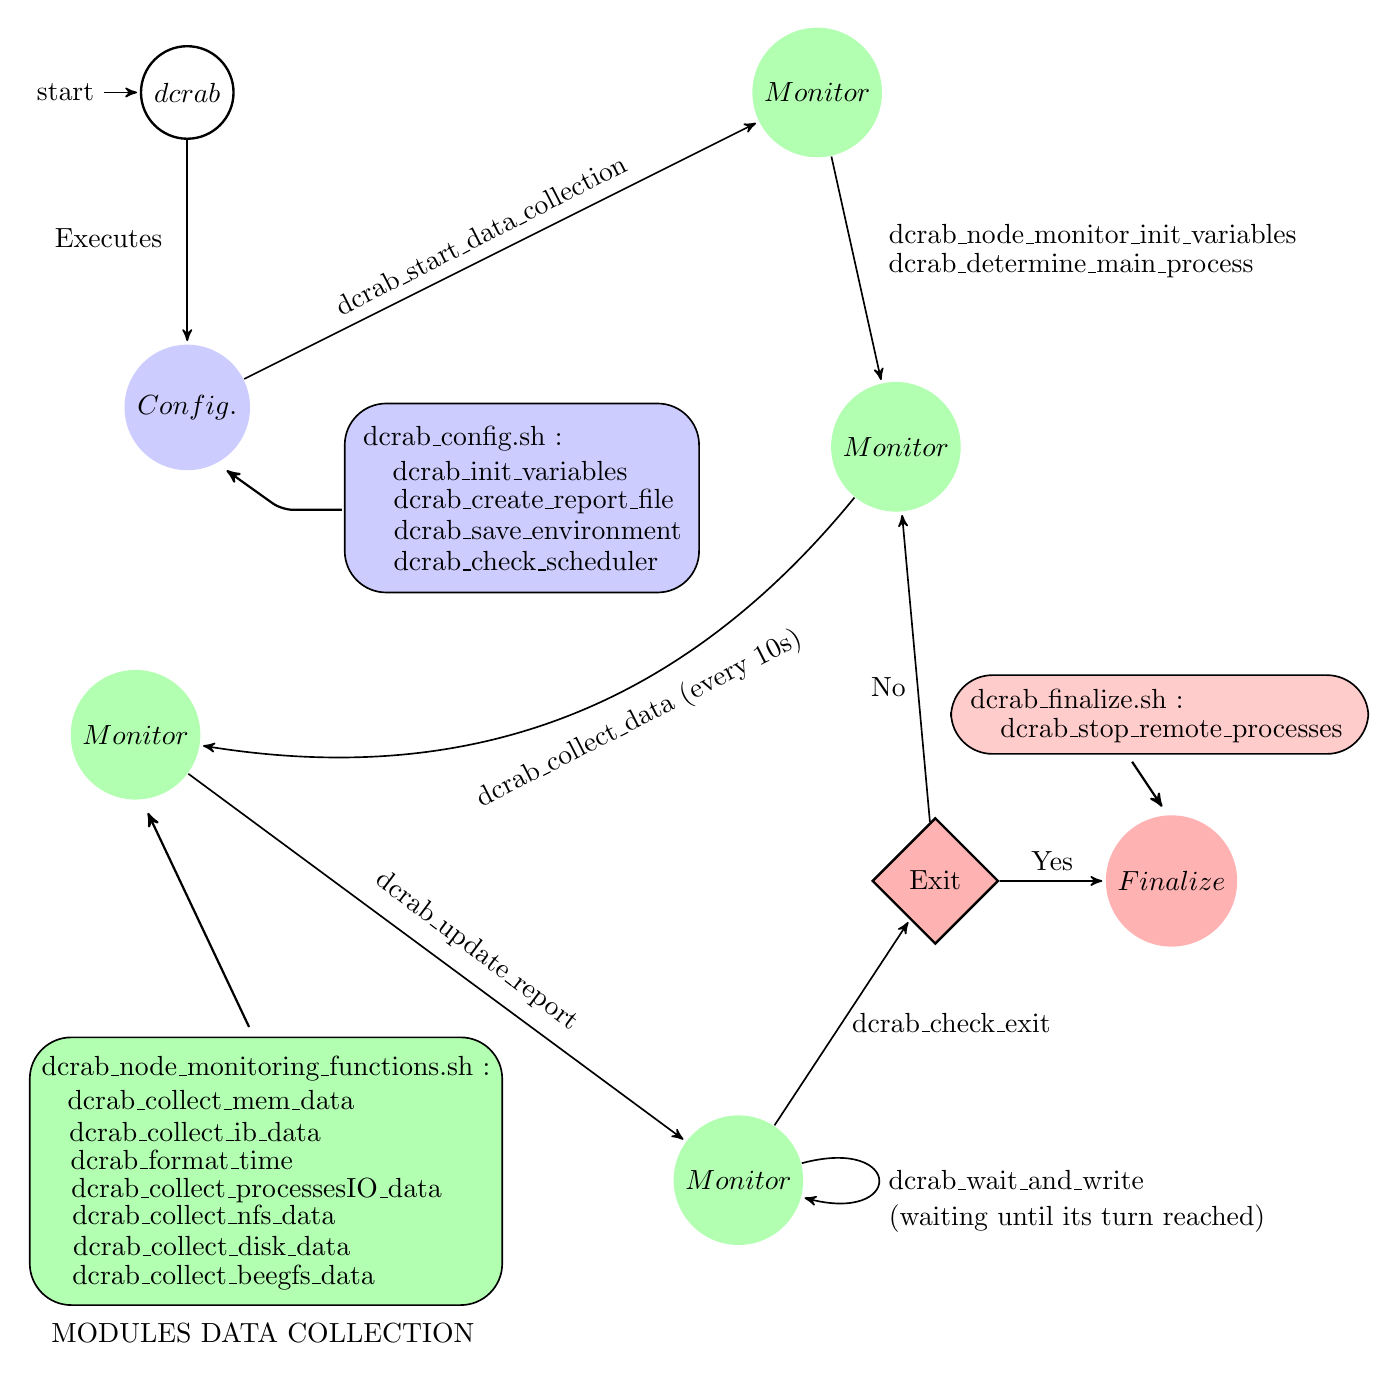
\begin{tikzpicture}[->,>=stealth',shorten >=1pt,auto,node distance=8cm,
                    semithick]
  \tikzstyle{every state}=[draw=none,text=black]

  \node[initial,state,draw,line width = 0.3mm] (A)              {$dcrab$};
	\node[state, node distance=4cm, fill=blue!20] 				 (B) [below of=A] {$Config.$};
  \node[state, fill=green!30]         (C) [right of=A] {$Monitor$};
	\node[state, node distance=2cm, xshift=1cm, yshift=-2.5cm, fill=green!30]         (D) [below of=C] {$Monitor$};
	\node[state, xshift=-4cm, yshift=2cm, fill=green!30]         (E) [below left of=D] {$Monitor$};
	\node[state, fill=green!30, xshift=2cm]         (F) [below right of=E] {$Monitor$};
	\node[state, draw, rectangle, minimum size=3.2em, line width = 0.3mm, xshift=-5.5cm, yshift=3.8cm, fill=red!30,  cm={cos(45) ,-sin(45) ,sin(45) ,cos(45) ,(0 cm,0 cm)}]         (G) [above right of=F] {};
	\node[state, node distance=3cm,  fill=red!30]         (H) [right of=G] {$Finalize$};

  \path (A) edge              node {} (B)
        (B) edge 							node {} (C)
				(C) edge 							node {} (D)
				(D) edge [bend left]	node {} (E)
				(E) edge 							node {} (F)
				(F) edge 						  node [right] {dcrab\_check\_exit} (G)
						edge [loop right] node {dcrab\_wait\_and\_write} (F)
				(G) edge 							node {No} (D)
				(G) edge 							node {Yes} (H);
\node[yshift=-1.85cm, xshift=-1cm] (t1) {Executes};

\filldraw[rounded corners=15pt, fill=blue!20, draw=black, node distance=0.4cm, yshift=-6.35cm, xshift=2cm] (0,0) rectangle (4.5,2.4);
\node[yshift=-4.4cm, xshift=3.5cm] (t2)   {dcrab\_config.sh :};
\node[node distance=0.4cm, xshift=0.6cm] (t3) [below of=t2] {dcrab\_init\_variables};
\node[node distance=0.4cm, xshift=0.3cm] (t4) [below of=t3]  {dcrab\_create\_report\_file};
\node[node distance=0.4cm, xshift=0.05cm, yshift=0.05cm] (t5) [below of=t4]  {dcrab\_save\_environment};
\node[node distance=0.4cm, xshift=-0.15cm] (t6) [below of=t5]  {dcrab\_check\_scheduler};
\draw [<-, rounded corners, thick, black, yshift=-5.3cm, xshift=1cm] (-0.5,0.5) -- (0.2,0) -- (1,0);

\node[yshift=0cm, xshift=11.5cm] (t9)   {};
\node[node distance=0.4cm, yshift=-1.4cm] (t10) [below of=t9] {dcrab\_node\_monitor\_init\_variables};
\node[node distance=0.4cm, xshift=-0.275cm] (t11) [below of=t10]  {dcrab\_determine\_main\_process};

\filldraw[rounded corners=15pt, fill=green!30, draw=black, yshift=-15.4cm, xshift=-2.0cm] (0,0) rectangle (6,3.4);
\node[yshift=-12.4cm, xshift=1cm] (t12)   {dcrab\_node\_monitoring\_functions.sh :};
\node[node distance=0.4cm, xshift=-0.7cm] (t13) [below of=t12] {dcrab\_collect\_mem\_data};
\node[node distance=0.4cm, xshift=-0.2cm] (t14) [below of=t13]  {dcrab\_collect\_ib\_data};
\node[node distance=0.4cm, xshift=-0.17cm, yshift=0.05cm] (t15) [below of=t14]  {dcrab\_format\_time};
\node[node distance=0.4cm, xshift=0.95cm] (t16) [below of=t15]  {dcrab\_collect\_processesIO\_data};
\node[node distance=0.4cm, xshift=-0.67cm, yshift=0.1cm] (t17) [below of=t16]  {dcrab\_collect\_nfs\_data};
\node[node distance=0.4cm, xshift=0.1cm] (t18) [below of=t17]  {dcrab\_collect\_disk\_data};
\node[node distance=0.4cm, xshift=0.15cm] (t19) [below of=t18]  {dcrab\_collect\_beegfs\_data};
\draw [<-, rounded corners, thick, black, yshift=-11.9cm, xshift=0.8cm] (-1.3,2.75) -- (0,0);
\node[node distance=0.4cm, yshift=-0.3cm,  xshift=0.5cm] (t20) [below of=t19]  {MODULES DATA COLLECTION};

\filldraw[rounded corners=15pt, fill=red!20, draw=black, yshift=-8.4cm, xshift=9.7cm] (0,0) rectangle (5.3,1);
\node[yshift=-7.7cm, xshift=11.3cm] (t21)   {dcrab\_finalize.sh :};
\node[node distance=0.4cm, xshift=1.2cm] (t22) [below of=t21] {dcrab\_stop\_remote\_processes};
\draw [->, rounded corners, thick, black, yshift=-8.5cm, xshift=12cm]  (0,0) -- (0.4, -0.6);

\node[cm={cos(27) ,sin(27) ,-sin(27) ,cos(27) ,(0 cm,0 cm)}, yshift=-3.3cm, xshift=2.5cm] (t80) {dcrab\_start\_data\_collection};
\node[cm={cos(27) ,sin(27) ,-sin(27) ,cos(27) ,(0 cm,0 cm)}, yshift=-9.7cm, xshift=1.5cm] (t81) {dcrab\_collect\_data (every 10s)};
\node[cm={cos(37) ,-sin(37) ,sin(37) ,cos(37) ,(0 cm,0 cm)}, yshift=-6.5cm, xshift=9.5cm] (t82) {dcrab\_update\_report};
\node[yshift=-10cm, xshift=9.5cm] (t83) {Exit};
\node[yshift=-14.3cm, xshift=11.3cm] (t84) {(waiting until its turn reached)};
\end{tikzpicture}
\caption{DCRAB's state machine}
\label{dcrabCodeScheme}
\end{figure}

Above, in the figure \ref{dcrabCodeScheme}, is presented a bit modificated state machine which presents the states where DCRAB passed through. Each node represents the main steps made by the tool and each edge an operation to change between states. There are boxes attached to some states to point the functions executed on them.

\begin{itemize}
  \item The first node, which is named as \verb+dcrab+, represents the script executed with \verb+dcrab start+ command.
  \item The second node \verb+Config.+ represents the configuration made by the tool where different functions are executed (attached box in blue color). It starts in each node the data collection.
  \item The next node \verb+Monitor+ is the first of four states that represent the process started in background on the compute nodes. This first node initialize some variables to execute correctly the data collection and creates the minimal environment to work. Among other things it will find the main process of the job which is and will be the parent of all the processes started by the job on that compute node. The tool take advantage of the scheduler used to identify that main process.
  \item The next \verb+Monitor+ node represents the moment where the update function will be executed to go to the next step. This node is the first node of the main loop made by the tool until the job finishes or crashes.
  \item This fiveth node starts with the update function and represents the data collection of every module implemented. In its box attached are written the names of the functions in charge of it. It prepares the data that will be written to go to the next step.
  \item In this last \verb+Monitor+ state, where the data will has been collected and prepared to write, a wait will be done until the write turn of the node reaches. For that purpose a mark have been inserted in the first line of the report to ensure any of the nodes writes until the last node updates have been made correctly. Normally the nodes do not wait more than a second to write into the report.

  On the other hand, in this state it checks the exit of the tools in some scenarios as described in the section \ref{crash}. If the conditions are satisfied it goes to the final state and if not it returns to the second \verb+Monitor+ state where another data collection will be done in the next \verb+DCRAB_COLLECT_TIME+ seconds.
  \item The last node, called \verb+Finalize+, is reached when some conditions are satisfied as described in \ref{crash} section. Here DCRAB finishes and is going to kill all DCRAB instances inside the compute nodes (those processes launched in background).
\end{itemize}

\chapter{Creating New Module}

The process to create a new module is straightforward. It could be divided into two main steps, the first one the step where you must make the module to collect wanted data, and the second one modify the html report to display the information collected. The second step is not a must so you can decide not to do and store the collected data into a file. You need to add a few lines in \texttt{dcrab\_node\_monitoring\_functions.sh} for the first part, and other lines into \texttt{dcrab\_report\_functions.sh} script to configure the display.

Below are presented the steps to insert a new module and the best way to name variables and functions in charge of it, however, the names are only a recommendation to preserve the coherence in the code.

\section{Step 1: Data collection}

The first thing to think about, in case you want to plot the collected data, is the type of chart you are going to use. DCRAB is going to upgrade the report file continuously by adding new data to the charts every loop, so you need to know how this data need to be inserted in the report. The charts we used are made with the \href{https://developers.google.com/chart/interactive/docs/reference}{Google Visualization API} so take a look to the documentation to choose one of them.

Once you have choosen one chart type, you have to understand the way you could insert data into them. Normally it consists in generate a string with the correct structure of the new point of the chart to be inserted. We normally store this data string in variables named \verb+DCRAB_MODULENAME_DATA+.

The changes that must be made in \texttt{dcrab\_node\_monitoring\_functions.sh} script are:

\begin{itemize}
  \item In the function \texttt{dcrab\_node\_monitor\_init\_variables()}: the variables needed for your module must be added where the \verb+## NEW MODULE CODE ##+ line is, that is, at the end of other variable declarations. You should use the naming we have used in all the variables of the tool which starts with \verb+DCRAB_+. A variable \verb+DCRAB_NEWMODULENAME_DATA+ should be created, which will be used to insert the data of the new module into the report file.
  \item Create a function, which should name as \texttt{dcrab\_collect\_newModuleName\_data()}, after the last module function defined, where the line \verb+## ADD NEW MODULE'S FUNCTION HERE ##+ is. Collect the data and fill up the variable \verb+DCRAB_NEWMODULENAME_DATA+ must be the purpose of this function. As we have pointed out, remember to generate properly the data on \verb+DCRAB_NEWMODULENAME_DATA+ variable. For example, in most of the cases we fill up the variable with a new point of the charts, which is translated to generate a string with the information of that point using the data collected (you could understand better looking how the data is inserted at the examples in \verb+/examples/normalReport/+ or in the \href{https://developers.google.com/chart/interactive/docs/reference}{Google Visualization API Documentation}).
  \item In the function \texttt{dcrab\_determine\_main\_process()} you have to add at the beginning, where the string \verb+## ADD INITIALIZATION OF NEW MODULE VARIABLE HERE ##+ is, the initialization of the \verb+DCRAB_NEWMODULENAME_DATA+ variable if needed. After that, at the bottom of the same function, add where the string \verb+## ADD THE CALL TO THE NEW FUNCTION HERE ##+ is, the call to the function \texttt{dcrab\_collect\_newModuleName\_data()} created.
  \item Finally, you must repeat the previous step inside the \texttt{dcrab\_collect\_data()} function in the same way.
\end{itemize}

\section{Step 2: Display}

This second step is only needed for display the data into the report, so do not do it if you do not want to visualize the data.

The changes that must be made in \texttt{dcrab\_report\_functions.sh} script are:

\begin{itemize}
  \item We previously store in a file the commands used to make the upgrade in the report and after we execute them at once. The function \texttt{dcrab\_write\_data()} is in charge of this operation and this is where you need to put your own lines: at the bottom of the function, where the string \verb+## NEW MODULE OPERATIONS ##+ is. Be sure to append the command in the file named \verb+DCRAB_COMMAND_FILE+ which will be execute later.
  \item In the function \texttt{dcrab\_generate\_html()} a few modifications need to be make: 1) At the message \verb+## NEW MODULE CODE 1##+ you have to add the data of the chart. 2) Where the message \verb+## NEW MODULE CODE 2 ##+ is you have to add the options of the chart as defined in \href{https://developers.google.com/chart/interactive/docs/reference}{Google Visualization API}. 3) At \verb+## NEW MODULE CODE 3 ##+ you have to create the chart object, call to the draw function and create a listener to be executed when ready event is fired (necessary to the correct drawing of the chart). 4) Add the tab of the new module at \verb+## NEW MODULE CODE 4 ##+. Copy the structure of the above tabs to generate the new one because the names of \verb+<li>+ tag's id, button tag's id and \texttt{tabChanges()} function's arguments must be named as there. 5) Where \verb+## NEW MODULE CODE 5 ##+. is you need to add the chart definition. The required lines to insert correctly the chart are shown below:

  \begin{verbatim}
  printf "%s \n" "<div id=\"processesIOChart\" class=\"chart\" style=\"disp-
  lay:block;\">" >> $DCRAB_HTML
  printf "%s \n" "<div class=\"overflowDivs\">" >> $DCRAB_HTML
  i=1
  while [ $i -le $DCRAB_NNODES ]; do
     printf "%s \n" "<div class=\"inline\">" >> $DCRAB_HTML
     printf "%s \n" "<table><tr><td>" >> $DCRAB_HTML
     printf "%s \n" "<div style=\"width: 1100px;\" class=\"header\">$(echo
     $DCRAB_NODES | cut -d' ' -f $i)</div>" >> $DCRAB_HTML
     printf "%s \n" "</td></tr>" >> $DCRAB_HTML
     printf "%s \n" "<tr><td>" >> $DCRAB_HTML

     #################################
     ## NEW MODULE CHART DEFINITION ##
     #################################

     printf "%s \n" "</td></tr>" >> $DCRAB_HTML
     printf "%s \n" "</table>" >> $DCRAB_HTML
     printf "%s \n" "</div>" >> $DCRAB_HTML
     i=$((i+1))
   done
   printf "%s \n" "</div>" >> $DCRAB_HTML
   printf "%s \n" "</div>" >> $DCRAB_HTML
\end{verbatim}


\end{itemize}


\chapter{Internal Report Operation}
\label{internalReportChapter}
This DCRAB's operation was implemented for sysadmins. DCRAB could monitor some aspects that the scheduler is not able to collect, so this operation mode allows the sysadmins to collect some of the data that only could be catch during the job's execution. Currently, at the 2.0 version, some of the modules added to this operation mode (infiniband and disk modules) are used in the normal mode, so the functions to collect the data are the same.

As the normal operation, it needs a folder to store the necessary files to make the communication between the compute nodes. That file path is set with the variable \verb+DCRAB_REPORT_DIR+, as the normal report operation, but it will point to another path and must be defined. This report directory will have the same structure as the normal operation one that is explained in \ref{dataCollection} section but it will only execute the modules added in this internal operation.

In this operation there is no real-time report generated because the user does not request it, so its not necessary. However, the data monitorized is going to be stored in a file to generate the report later. That file, which is set with the \verb+DCRAB_IREPORT_DATA_FILE+ variable, is going to be written only by the main node. The rest of the nodes will store its own data in the folders used to write and the main node will collect their data to write into the file pointed by \verb+DCRAB_IREPORT_DATA_FILE+.

The idea of this mode is to be transparent for the user. If the user decide to not execute DCRAB in his/her job the sysadmin could insert in his/her submission script the lines described in \ref{internalReport} to execute DCRAB in internal operation mode. For this purpose was created the file \texttt{/auxFiles/dcrab\_PBS\_comprobation.sh}.

\section{Activate Internal Report}
\label{internalReport}
The way to activate this operation mode is similar to the normal one:

\ \

\begin{verbatim}
    export DCRAB_PATH=/PATH_TO_DCRAB/src/
    export PATH=$PATH:$DCRAB_PATH
    dcrab istart

    ##################################
    #    BLOCK OF CODE TO MONITOR    #
    ##################################

    dcrab ifinish
\end{verbatim}

Notice that an extra '\verb+i+' must be added to the \verb+start+ and \verb+finish+ commands.

\section{Code Explanation and Customization}

There is not to much to explain in this part, because the core of the internal operation is the same as the normal operation one, however, there are some details that must me pointed. The scripts which compose this operation are:

\begin{itemize}
  \item \texttt{dcrab\_internal\_report\_functions.sh} with two functions: 1) \texttt{dcrab\_internal\_report}- \texttt{\_init\_variables()} to initialize the variables needed for the report and 2) \texttt{dcrab\_write\_internal\_data()} to write into the file that will store the data collected, which is pointed by \verb+DCRAB_IREPORT_DATA_FILE+. This function is going to be executed only by the main node.
  \item \texttt{dcrab\_internal\_report\_generation.sh} which is used to generate the internal report with all the files created per job (with the \verb+DCRAB_IREPORT_DATA_FILE+ variable). This script is adapted to our particular case, so you could create your own one to visualize the data collected with this internal operation mode in the way you want to. However, we will detail the variables you need to change to adapt this script to your own scenario in case you want to use it (in \ref{internalReportCustomization} section).
\end{itemize}

\section{Internal Report Customization}
\label{internalReportCustomization}

There are some variables which may be customize in the internal report:

\begin{itemize}
  \item \texttt{DCRAB\_IREPORT\_DATA\_FILE} inside \texttt{dcrab\_internal\_report\_init\_variables()} function of \verb+dcrab_internal_report_functions.sh+ script. It is used to store the data monitorized. It will be only written by the main node.
  \item \texttt{DCRAB\_REPORT\_DIR} inside \texttt{dcrab\_init\_variables()} function in \verb+dcrab_config.sh+ script. In the case of the internal report it is used to configure the path to the reporting file.
\end{itemize}

And here the variables defined in \texttt{dcrab\_internal\_report\_generation.sh} which you could customize to adapt the script to your case and generate the internal report:

\begin{itemize}
  \item \texttt{DCRAB\_IREPORT} which is the path to the internal report file.
  \item \texttt{DCRAB\_IREPORT\_DATA\_DIR} which define the path where the files pointed by \verb+DCRAB_IREPORT_DATA_FILE+ are been generated. For example, if \verb+DCRAB_IREPORT_DATA_FILE+ is defined as \verb+/home/user/dcrab/data/JOBID+ the \verb+DCRAB_IREPORT_DATA_DIR+ variable must be defined as \verb+/home/user/dcrab/data+.
  \item \texttt{DCRAB\_IREPORT\_DATA\_BACKUP\_DIR} define the directory of the data backup. This variable's usage is explained deeper in \ref{intReportAuxScripts} section.
  \item \texttt{DCRAB\_NUMBER\_OF\_BARS} which defined the number of bars to appear in the plot.
  \item \texttt{DCRAB\_NUMBER\_OF\_CHARACTERS} is used to control the width of the progress bar displayed during the execution of the script (it is just an esthetic feature, you do not need to change it).
\end{itemize}

\section{Auxiliary Scripts}
\label{intReportAuxScripts}

There are a few more scripts implemented to make some operations on the internal report:

\begin{itemize}
  \item \texttt{dcrab\_internal\_report\_clean.sh} which recollects all the data generated by all the DCRAB jobs into one file to decrease the number of folders. Furthermore, it makes a tarball of all those files and their report folder and will save it in the directory pointed by \texttt{DCRAB\_IREPORT\_DATA\_BACKUP\_DIR} variable. It also removes the bad files, which may be generated from exited or crashed jobs.
  \item \texttt{dcrab\_PBS\_comprobation.sh} is used to insert into users' jobs script the required lines to execute DCRAB in internal operation mode on PBS scheduler type file. This script modify the file entered as the first argument and prepares it to submmit to the scheduler. It also checks a few scenarios where the user forgets some lines of DCRAB and trys to fix the file. Example of usage:

\begin{verbatim}
./dcrab_PBS_comprobation.sh script.pbs  --> Modifies script.pbs file as below
\end{verbatim}
\end{itemize}

\pagebreak

\begin{multicols}{2}
\begin{verbatim}
BEFORE

#!/bin/bash
#PBS -q parallel
#PBS -l nodes=1:ppn=24
#PBS -l mem=150gb
#PBS -l cput=1000:00:00
#PBS -N daniTestJob

module load QuantumESPRESSO
cd $PBS_O_WORKDIR

mpirun -np 24 pw.x < ausurf.in >& OUT

\end{verbatim}

\columnbreak

\begin{verbatim}

AFTER

#!/bin/bash
#PBS -q parallel
#PBS -l nodes=1:ppn=24
#PBS -l mem=150gb
#PBS -l cput=1000:00:00
#PBS -N daniTestJob
export DCRAB_PATH=/home/user/dcrab/software/src/
export PATH=$PATH:$DCRAB_PATH
dcrab istart

module load QuantumESPRESSO
cd $PBS_O_WORKDIR

mpirun -np 24 pw.x < ausurf.in >& OUT

dcrab ifinish
\end{verbatim}
\end{multicols}


\end{document}
